\chapter{TASK\_1.}

\textbf{Цель работы:}

\begin{itemize} 
	\item 
\end{itemize}

\textbf{Задание 1}


\begin{lstlisting}[caption=Код программы. TASK\_1. Главнвая функция main]
	
\end{lstlisting}

\begin{lstlisting}[caption=Код программы. TASK\_1. Реализация заданий]
	
\end{lstlisting}


\textbf{Вывод:}

\begin{itemize} 
	\item Были изучены
\end{itemize}

\textbf{Пример работы:}

% \begin{figure}[ht!]
% 	\centering{
% 		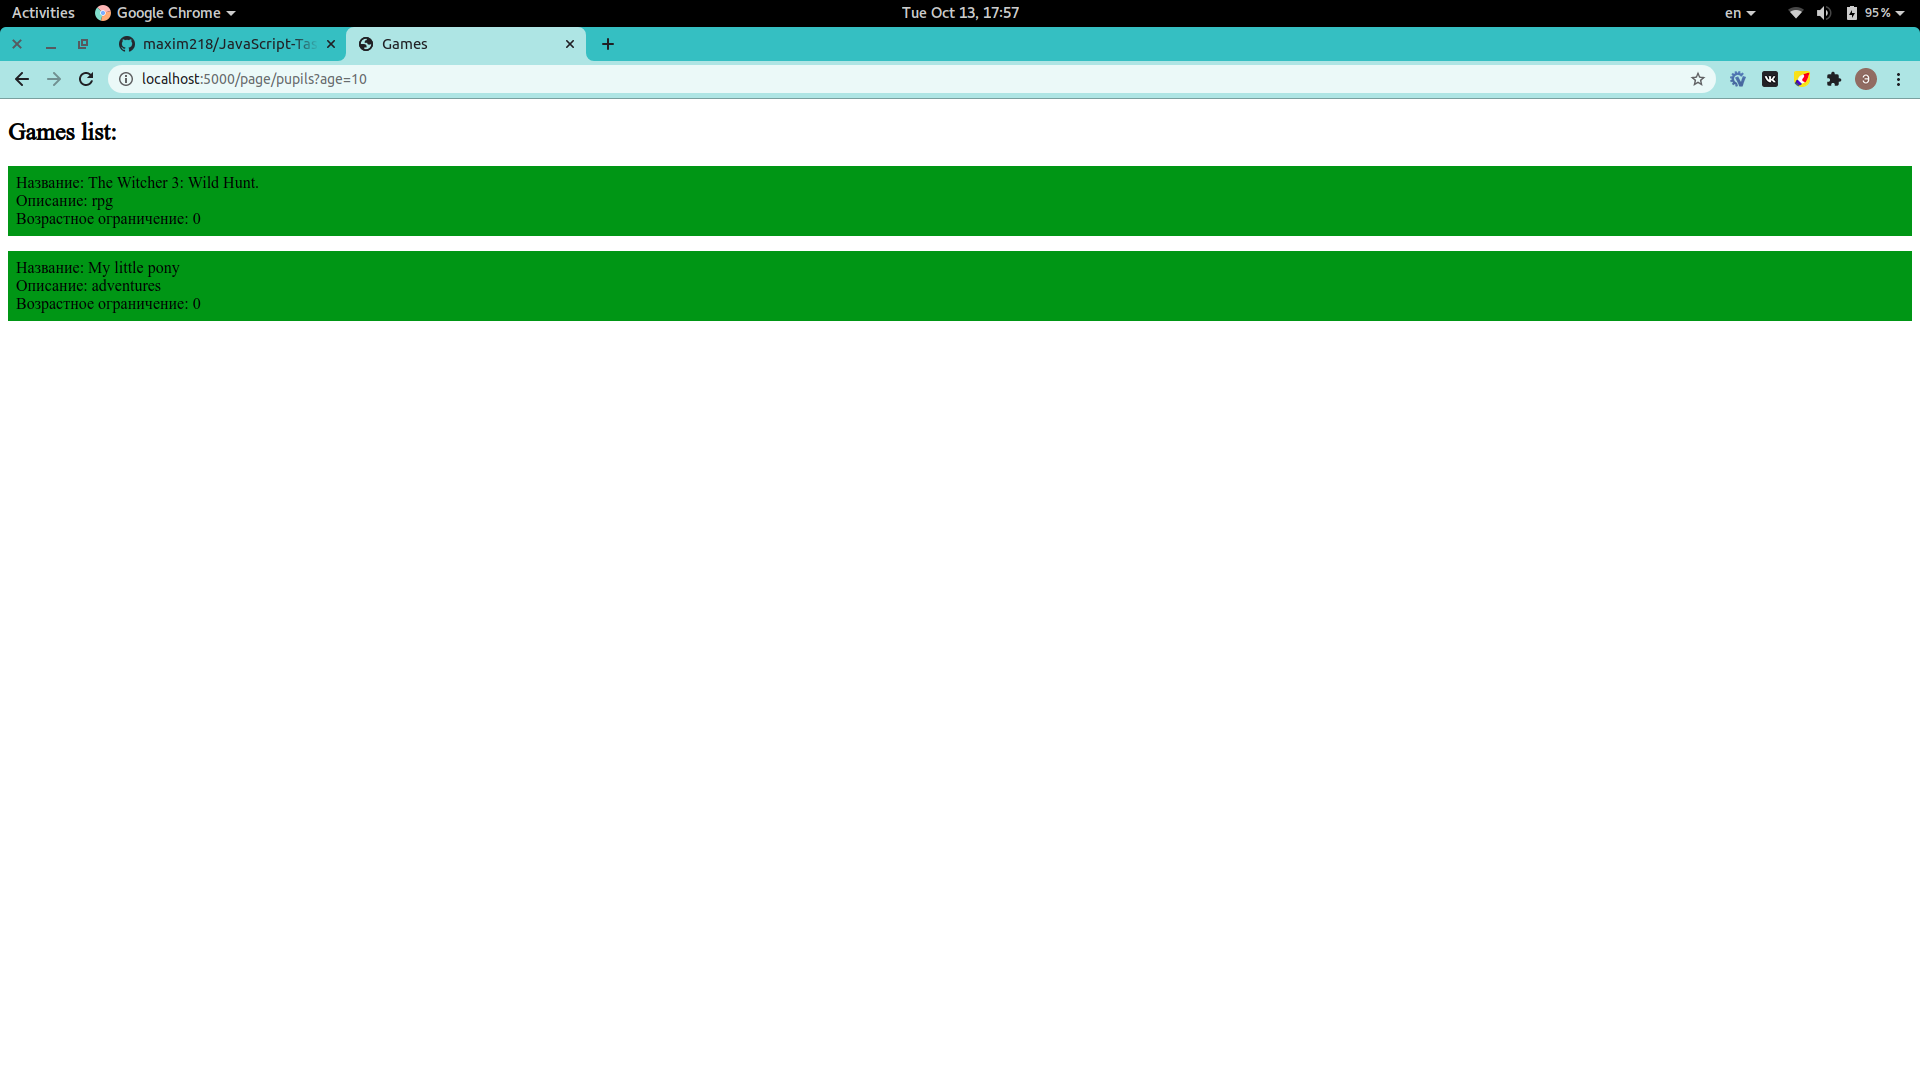
\includegraphics[width=0.9\textwidth]{img/1.png}
% 		\caption{Пример работы программы}}
% \end{figure}


\chapter{TASK\_2.}

\textbf{Цель работы:}

\begin{itemize} 
	\item 
\end{itemize}

\textbf{Задание 1}

\begin{lstlisting}[caption=Код программы. TASK\_2. Реализация заданий]

\end{lstlisting}


\textbf{Вывод:}

\begin{itemize} 
	\item 
\end{itemize}


\textbf{Пример работы:}

% \begin{figure}[ht!]
% 	\centering{
% 		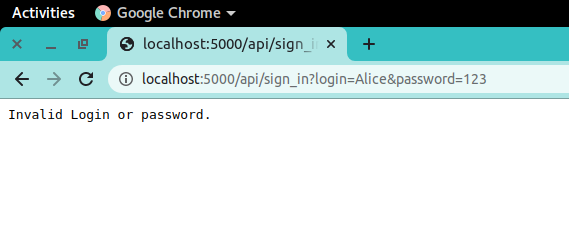
\includegraphics[width=0.9\textwidth]{img/3.png}
% 		\caption{Пример работы программы}}
% \end{figure}
